\section{Overview}

\begin{figure}[H]
        \centering 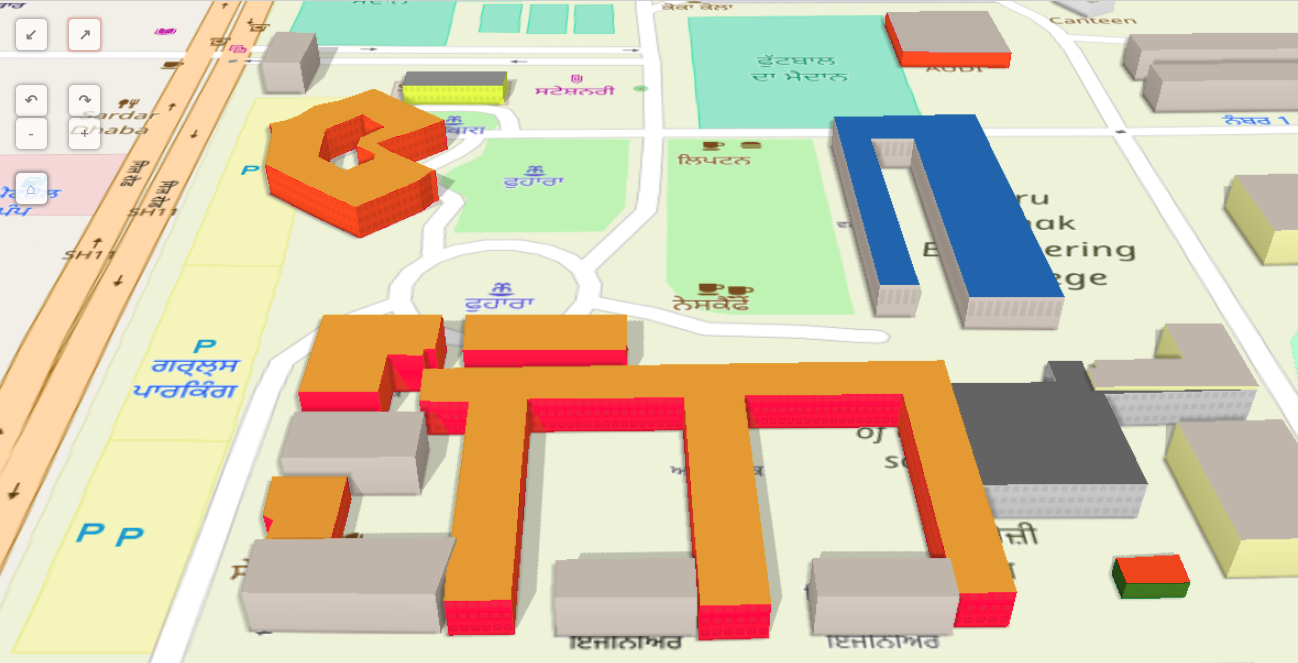
\includegraphics[scale=0.31]{input/images/osm_building.png}
        \caption{OpenStreetMap}
        \label{fig:openscadlogo}
\end{figure}

OpenStreetMap (OSM) is an open-source, free web-based software, owned by you, the contributors.OpenStreetMap is an online open data platform to collect the world's geographic data based on the Wikipedia model of crowdsourcing. The project started in 2004 by Steve Coast and is now governed by the non profit OpenStreetMap Foundation based in the UK.\\ 


OpenStreetMap is a free editable map of the whole world. It is made by people like you.” Which
means the database will always be subject to the whims, experimentation, and mistakes of the
community. This is precisely OSM’s strength since, among other things, it allows our data to
quickly accommodate changes in the physical world.


By making your system an OSM tile server not only you can edit the map but can use it offline
also. You can change the styling of the map like color of the roads fonts style and amny more as
per your requirments.\\


The core part of OSM is implemented using Mapnik library and database for rendering, mod\_tile and slippy
for web interface. Bash Shell Scripting has been used to automate the installation.


My training being not based on particular language or technology, different type of open-source softwares and technologies are
used in this project and many during my training which are not used in this
project like CGI (for web interface through c++).

\section{The Existing System}
Geographical data (geo data) is not free in many parts of the world.If you collect data from Google Maps in this way, you are creating a "derived work". Any such data retains the copyright conditions of the original. In practice, this means your data is subject to the licensing fees, and contractual restrictions, of these map providers. That's exactly what OpenStreetMap is trying to avoid. The data is copyrighted and owned by multiple organisations like the Ordnance Survey. Google/whoever just licenses it. If we were to use it, we'd have to pay for it.\\ 

In areas where there are no such data sources (most areas) we have to start from a blank slate, and head out there to survey the streets ourselves. Despite starting from scratch, we have achieved a good level of completion in many places.  

"Also, you may not use Google Maps in a manner which gives you or any other person access to mass downloads or bulk feeds of numerical latitude and longitude coordinates."

{\bf {Limitations of existing system }}
\begin{itemize}
\item We can't edit the maps.

\item Data may be inaccurate.

\item They are costly.

\item Can't create own map server.

\item Mass downloads or bulk feeds of numerical latitude and longitude coordinates is sometime impossible.
\end{itemize}

\section{User Requirement Analysis}
For User Requirement Analysis, users of this system have been asked about
possible requirements that this software should have and we got following
resultant list of outputs-:
\begin{enumerate}
\item A full editing history is stored for each user.
\item Provide on-line way to analysis so that individual does not have to
install anything.
\item Users can attach Wikipedia-like edit summaries to their edits, and there is a History tab on the main page that shows recent edits to the selected area.
\item The user can download the data in *.pbf or *.osm file format.
\item There is a help centre at help.openstreetmap.org.
\item Both techinal and non-technical users can use OSM.
\item User can make own OSM tile server.
\item User can run script for automatic installation.
\item To view the map on web browser.

\end{enumerate}



\section{Feasibilty Study}
This review is made to see if the project on completion will serve the purpose of the organization for the amount of work, effort and the time that spend on it. Feasibility study lets the developer foresee the future of the project and the usefulness. A feasibility study of a system proposal is according to its workability, which is the impact on the organization, ability to meet their user needs and effective use of resources. Carrying out a feasibility study involves information assessment, information collection and report writing. The information assessment phase identifies the information that is required to answer the three questions set out above. Once the information has been identified, you should question information sources to discover the answers to these questions Thus when a new application is proposed it normally goes through a feasibility study before it is approved for development.\\

A feasibility study is designed to provide an overview of the primary issues related to a business idea. The purpose is to identify any make or break issues that would prevent your business from being successful in the marketplace.\\%In other words, a feasibility study determines whether the business idea makes sense. A thorough feasibility analysis provides a lot of information necessary for the business plan.For example, a good market analysis is necessary in order to determine the project's feasibility.This information provides the basis for the market section of the business plan.\\\\

The document provide the feasibility of the project that is being designed and lists various areas that were considered very carefully during the feasibility study of this project such as Technical, Economic and Operational feasibilities.Feasibility is defined as the practical extent to which a project can be performed successfully. To evaluate feasibility, a feasibility study is performed, which determines whether the solution considered to accomplish the requirements is practical and workable in the software. Information such as resource availability, cost estimation for software development, benefits of the software to the organization after it is developed and cost to be incurred on its maintenance are considered during the feasibility study. The objective of the feasibility study is to establish the reasons for developing the software that is acceptable to users, adaptable to change and conformable to established standards.\\
Objectives of feasibility study are listed below:
\begin{itemize}
	\item To analyze whether the software will meet organizational requirements.
	\item To determine whether the software can be implemented using the current technology and within the specified budget and schedule.
	\item To determine whether the software can be integrated with other existing software.
\end{itemize}

\subsection{Types of Feasibility Study}
Various types of feasibility that are commonly considered include technical feasibility, economic feasibility, and behaviourial feasibility.

\subsubsection{Technical Feasibility}
Technical feasibility is one of the first studies that must be conducted after the project has been identified. In large engineering projects consulting agencies that have large staffs of engineers and technicians conduct technical studies dealing with the projects. In individual agricultural projects financed by local agricultural credit corporations, the technical staff composed of specialized agricultural engineers, irrigation and construction engineers, and other technicians are responsible for conducting such feasibility studies.\\ The Technical feasibility assessment is focused on gaining an understanding of the present technical resources of the organization and their applicability to the expected needs of the proposed system. It is an evaluation of the hardware and software and how it meets the need of the proposed system. This assessment is based on an outline design of system requirements, to determine whether the company has the technical expertise to handle completion of the project. When writing a feasibility report, the following should be taken to consideration:
\begin{itemize}
	\item A brief description of the business to assess more possible factors which could affect the study
	\item The part of the business being examined
	\item The human and economic factor
	\item The possible solutions to the problem
\end{itemize}

The system must be evaluated from the technical point of view first. The assessment of this feasibility must be based on an outline design of the system requirement in the terms of input, output, programs and procedures. Having identified an outline system, the investigation must go on to suggest the type of equipment, required method developing the system, of running the system once it has been designed. Technical feasibility assesses the current resources (such as hardware and software) and technology, which are required to accomplish user requirements in the software within the allocated time and budget. For this, the software development team ascertains whether the current resources and technology can be upgraded or added in the software to accomplish specified user requirements. A Technical feasibility also performs the following tasks.

\begin{itemize}
	\item Analyzes the technical skills and capabilities of the software development team members
	\item Determines whether the relevant technology is stable and established
	\item Ascertains that the technology chosen for software development has a large number of users so that they can be consulted when problems arise or improvements are required.
\end{itemize}

Technical issues raised during the investigation are:
\begin{itemize}
	\item Does the existing technology sufficient for the suggested one?
	\item Can the system expand if developed?
\end{itemize}

The project should be developed such that the necessary functions and performance are achieved within the constraints. The project is developed within latest technology. Through the technology may become obsolete after some period of time, due to the fact that never version of same software supports older versions, the system may still be used. So there are minimal constraints involved with this project. The system has been developed using Java the project is technically feasible for development.

OpenStreetMap is technically feasible as it is built up using various open source technologies and it can run on any platform.

\subsubsection{Economic Feasibility}
The purpose of the economic feasibility assessment is to determine the positive economic benefits to the organization that the proposed system will provide. It includes quantification and identification of all the benefits expected. This assessment typically involves a cost/ benefits analysis.\\

Economic feasibility is the cost and logistical outlook for a business project or endeavor. Prior to embarking on a new venture, most businesses conduct an economic feasibility study, which is a study that analyzes data to determine whether the cost of the prospective new venture will ultimately be profitable to the company. Economic feasibility is sometimes determined within an organization, while other times companies hire an external company that specializes in conducting economic feasibility studies for them.\\

The purpose of business in a capitalist society is to turn a profit, or to earn positive income. While some ideas seem excellent when they are first presented, they are not always economically feasible. That is, that they are not always profitable or even possible within a company's budget. Since companies often determine their budget's several months in advance, it is necessary to know how much of the budget needs to be set aside for future projects. Economic feasibility helps companies determine what that dollar amount is before a project is ultimately approved. This allows companies to carefully manage their money to insure the most profitable projects are undertaken. Economic feasibility also helps companies determine whether or not revisions to a project that at first seems unfeasible will make it feasible.\\

The developing system must be justified by cost and benefit. Criteria to ensure that effort is concentrated on project, which will give best, return at the earliest. One of the factors, which affect the development of a new system, is the cost it would require. Economic feasibility determines whether the required software is capable of generating financial gains for an organization. It involves the cost incurred on the software development team, estimated cost of hardware and software, cost of performing feasibility study, and so on. For this, it is essential to consider expenses made on purchases (such as hardware purchase) and activities required to carry out software development. In addition, it is necessary to consider the benefits that can be achieved by developing the software. Software is said to be economically feasible if it focuses on the issues listed below.
\begin{itemize}
	\item Cost incurred on software development to produce long-term gains for an organization.
	\item Cost required to conduct full software investigation (such as requirements elicitation and requirements analysis).
	\item Cost of hardware, software, development team, and training.
\end{itemize}

The following are some of the important financial questions asked during preliminary investigation:
\begin{itemize}
	\item The costs conduct a full system investigation.
	\item The cost of the hardware and software.
	\item The benefits in the form of reduced costs or fewer costly errors.
\end{itemize}

Since the system is developed as part of project work, there is no manual cost to spend for the proposed system. Also all the resources are already available, it give an indication of the system is economically possible for development.

\subsubsection{Behavioral Feasibility}
Behavioral feasibility assesses the extent to which the required software performs a series of steps to solve business problems and user requirements. It is a measure of how well the solution of problems or a specific alternative solution will work in the organization. It is also measure of how people feel about the system. If the system is not easy to operate, than operational process would be difficult. The operator of the system should be given proper training. The system should be made such that the user can interface the system without any problem.\\

Operational feasibility is a measure of how well a proposed system solves the problems, and takes advantage of the opportunities identified during scope definition and how it satisfies the requirements identified in the requirements analysis phase of system development. The operational feasibility assessment focuses on the degree to which the proposed development projects fits in with the existing business environment and objectives with regard to development schedule, delivery date, corporate culture, and existing business processes.\\

To ensure success, desired operational outcomes must be imparted during design and development. These include such design-dependent parameters such as reliability, maintainability, supportability, usability, producibility, disposability, sustainability, affordability and others. These parameters are required to be considered at the early stages of design if desired operational behaviors are to be realized. A system design and development requires appropriate and timely application of engineering and management efforts to meet the previously mentioned parameters. A system may serve its intended purpose most effectively when its technical and operating characteristics are engineered into the design. Therefore, operational feasibility is a critical aspect of systems engineering that needs to be an integral part of the early design phasesThis feasibility is dependent on human resources (software development team) and involves visualizing whether the software will operate after it is developed and be operative once it is installed. Operational feasibility also performs the following tasks.\\

\begin{itemize}
	\item Determines whether the problems anticipated in user requirements are of high priority.
	\item Determines whether the solution suggested by the software development team is acceptable.
	\item Analyzes whether users will adapt to a new software.
	\item Determines whether the organization is satisfied by the alternative solutions proposed by the software development team.
\end{itemize}

This includes the following questions:
\begin{itemize}
	\item Is there sufficient support for the users?
	\item Will the proposed system cause harm?
	\item The project would be beneficial because it satisfies the objectives when developed and installed. All behavioral aspects are considered carefully and conclude that the project is behaviorally feasible.
\end{itemize}

\section{Objective of Project }
The main objective of this project is to help GNE freshers to locate the places like labs, Admin Block, TCC etc from phone or laptop easily. The map is provided in Punjabi language. They can easily search the place by typing in the search button. In order to entertain them, the projects includes animations, GNE Tour and lot more. 
\begin{enumerate}
\item The map includes 3-D View with the shadows of buildings.
\item Styling of the map by adding international boundary of India.
\item Automation for making the system an OSM tile server.
\end{enumerate}

